\documentclass[handout,10pt]{beamer}

\usetheme{AnnArbor}
\usecolortheme{beaver}

\graphicspath{{include/}}

\setlength{\unitlength}{\textwidth}  % measure in textwidths
\usepackage[normalem]{ulem}
\usepackage{colortbl}
% to avoid counting all pages
\newcommand{\backupbegin}{
   \newcounter{finalframe}
   \setcounter{finalframe}{\value{framenumber}}
}
\newcommand{\backupend}{
   \setcounter{framenumber}{\value{finalframe}}
}


\setbeamertemplate{navigation symbols}{}
\setbeamertemplate{enumerate items}[default]
\setbeamertemplate{enumerate subitem}{\alph{enumii}.}
\setbeamertemplate{enumerate subsubitem}{\roman{enumiii}.}
\setkeys{Gin}{width=0.6\textwidth}

\newcommand{\ind}{\stackrel{ind}{\sim}}
\providecommand{\ov}[1]{\overline{#1}}


\institute[ISU]{Iowa State University}
\date{\today}

\title[Empirical Bayesian Method vs. Other Methods]{Differential Expression Analysis Methods Comparison}
\author{Xiyuan Sun}

\usepackage{Sweave}
\begin{document}
\Sconcordance{concordance:presentation.tex:presentation.Rnw:%
1 36 1 1 0 377 1}


\begin{frame}
\maketitle

\pause

\vspace{0.2in} \pause

{\tiny
This research was built on Niemi et al's approach (Niemi et al., 2015). Their research was supported by National Institute of General Medical Sciences (NIGMS) of the National Institutes of Health and joint National Science Foundation / NIGMS Mathematial Biology Program under award number R01GM109458. 
}

\end{frame}





\begin{frame}
\frametitle{Outline}

\begin{itemize}
\item Background
	\begin{itemize}
	\item RNA-seq procedure
	\item RNA-seq data
	\item Differential Expression (DE) Analysis
	\end{itemize}
\item Modeling 
	\begin{itemize}
	\item Negative Binomial Model in Generalized Linear Model 
	\item Hierarchical overdispersed count regression model 
	\item Null hypotheis for DE analysis
	\end{itemize}
\item Inference
	\begin{itemize}
	\item Empirical Bayes
	\item Alternative Methods
	\end{itemize}
\item Simulation studies
	\begin{itemize}
	\item DE Genes detection via ROC curves
	\item Area under ROC curve values
	\end{itemize}
%\item Ongoing work
\end{itemize}

\end{frame}


\section{Background}
\subsection{RNA-seq procedure}

\begin{frame}
\frametitle{RNA fragmentation, sequencing, and alignment}
\setkeys{Gin}{width=0.5\textwidth}
\begin{center}
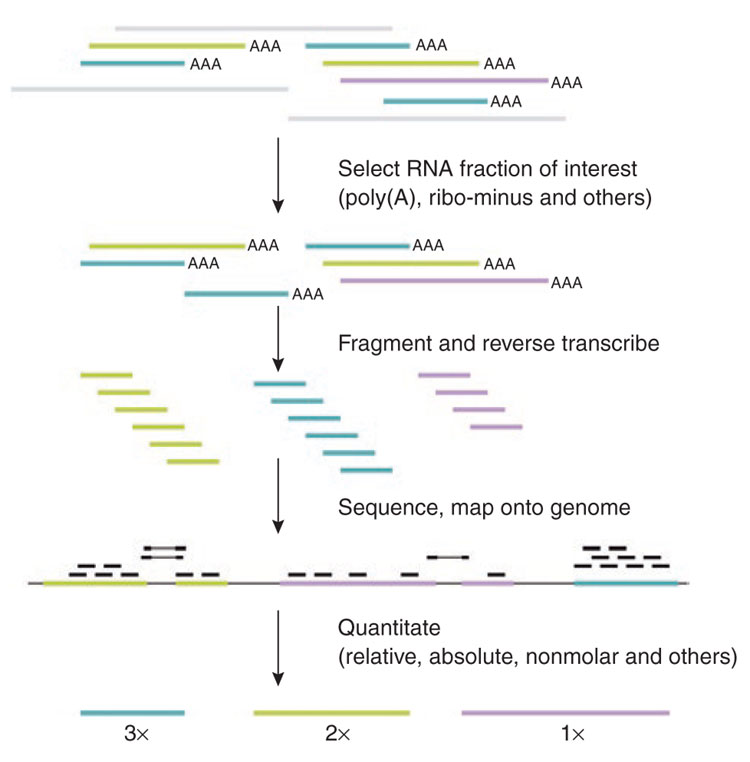
\includegraphics{rnaseq3}
\end{center}
{\tiny (Pepke, Wold, and Mortazavi (2009) \url{http://www.nature.com/nmeth/journal/v6/n11s/fig_tab/nmeth.1371_F5.html})}
\end{frame}

\subsection{RNA-seq data}
\begin{frame}
\frametitle{RNAseq data}
\begin{table}[ht]
\centering
\resizebox{\columnwidth}{!}{%
\begin{tabular}{|r|r|r|r|r|>{\columncolor[gray]{0.8}}r|>{\columncolor[gray]{0.8}}r|>{\columncolor[gray]{0.8}}r|>{\columncolor[gray]{0.8}}r|}
  \hline
 Genes & B73 & B73 & B73 & B73 & Mo17 & Mo17 & Mo17 & Mo17 \\ 
 & Rep1 & Rep2 & Rep3 & Rep4 & Rep1 & Rep2 &Rep3 & Rep4\\
  \hline
\textbf{AC148152.3\_FG001} &   3 &   4 &   6 &   0 &   8 &  17 &  18 &  20 \\ 
  \textbf{AC148152.3\_FG008} &   3 &   3 &   4 &   1 &  31 &  40 &  45 &  49 \\ 
  \textbf{AC152495.1\_FG002} &  33 &  46 &  18 &  13 &   4 &   0 &   2 &   6 \\ 
  \textbf{AC152495.1\_FG017} &  41 &  44 &  16 &  13 &   2 &   2 &   2 &   0 \\ 
  \textbf{AC184130.4\_FG012} &  24 &  47 &  18 &  21 & 110 & 144 & 121 &  96 \\ 
  \textbf{AC184133.3\_FG001} &   0 &   1 &   1 &   0 &  14 &  13 &   4 &   9 \\ 
   \hline
   \hline
AC148152.3\_FG005 & 2323 & 1533 & 1932 & 1945 & 2070 & 1582 & 2196 & 1882 \\ 
  AC148167.6\_FG001 & 672 & 598 & 728 & 713 & 743 & 655 & 821 & 824 \\ 
  AC149475.2\_FG002 & 459 & 438 & 451 & 483 & 467 & 448 & 634 & 532 \\ 
  AC149475.2\_FG003 & 1184 & 976 & 1131 & 1206 & 891 & 743 & 1288 & 1107 \\ 
  AC149475.2\_FG005 & 551 & 535 & 360 & 353 & 550 & 524 & 492 & 440 \\ 
  AC149475.2\_FG007 & 245 & 214 & 169 & 159 & 297 & 262 & 210 & 302 \\ 
   \hline
\end{tabular}%
}
\end{table}

\pause
{\small
\begin{itemize}
\item DE genes: expression in Genotype Variety $B73$ is different from that in another Genotype Variety $Mo17$
\end{itemize}
}

\end{frame}


\subsection{DE Analysis}
\begin{frame}
\frametitle{Differential Expression Genes}
\begin{definition}
A gene is regarded as differentially expressed (DE) when the expected count reads of this gene corresponding to one genotype variety differs from that of another genotype variety. 
\end{definition}

\pause
\begin{center}
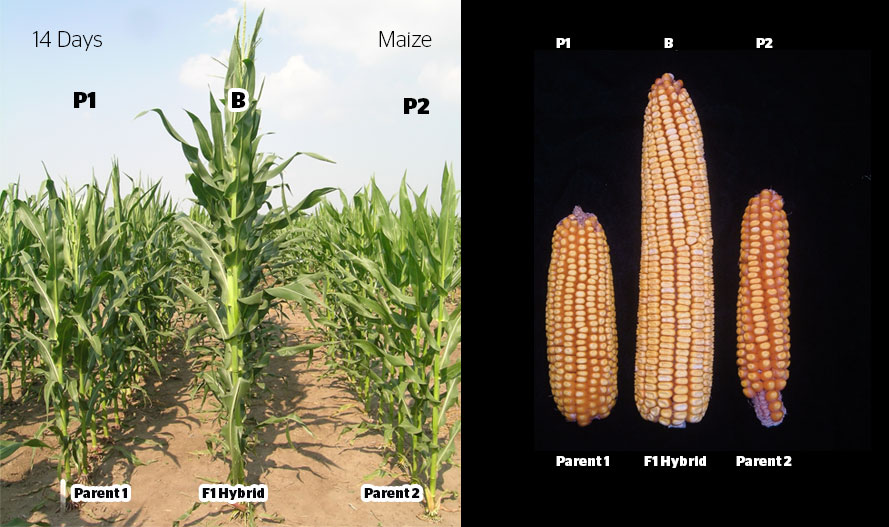
\includegraphics{heterosis}
\end{center}

{\tiny (\url{http://www2.iastate.edu/~nscentral/news/06/may/vigor.shtml} modified by Will Landau)} 
\end{frame}


\begin{frame}
\frametitle{Differential expression analysis}

\begin{definition}
For a given gene, we use statistical testing to decide whether an observed difference in read counts is significant, i.e., whether it is greater than what would be expected just due to natural random variation.
\end{definition}

\begin{itemize}
\item Normalization

Estimated normalization factors should ensure that a gene with the same expression level in two samples is not detected as DE. 
\item Assumed distribution

Negative binomial

\item Parameter estimation

Mean, Dispersion

\item Test for DE

Exact test, Wald test, t-test

\end{itemize}

\end{frame}


\section{Modeling}

\subsection{Negative Binomial Model in Generalized Linear Model}

\begin{frame}
\frametitle{Negative Binomial Model in Generalized Linear Model Framework (Part 1)}

Let 
\begin{itemize}
\item $g$ ($g=1,\ldots,G$) identify the gene, 
\item $i$ ($i=1,2$) identify the genotype variety, 
\item $j$ ($j=1,2,3,4$)
\item $Y_{gij}$ be the RNAseq counts of gene $g$, genotype variety $i$, replicate $j$
\end{itemize}
\pause
We assume 
\begin{equation}
Y_{gij} \ind \text{NB} \left (\mu_{gij}, \phi_g \right )
\end{equation}
where 
\begin{itemize}[<+->]
\item $\mu_{gij}$ are means of read counts of gene $g$ genotype $i$ replicate $j$,
\item $\phi_{g}$ allow for gene-specific overdispersion
\end{itemize}
\end{frame}

\begin{frame}
\frametitle{Negative Binomial Model in Generalized Linear Model Framework (Part 2)}

In the generalized linear model (GLM) setting, the mean response, $\mu_{gij}$ is linked to a linear predictor with natural log link:

\begin{equation}
log(\mu_{gij}) = x_{i}^T \beta_g + log(N_{ij})
\end{equation}
where 
\begin{itemize}[<+->]
\item $x_{i}$ is row of the design matrix containing the covariates indicating this sample belongs to variety $i$,
\item $\beta_g = (\beta_{g1}, \beta_{g2})$ is a vector of regression parameters
\item $N_{ij}$ is the normalized library size of replicate $j$ in variety $i$
\end{itemize}

\end{frame}




\subsection{Hierarchical overdispersed count regression model}

\begin{frame}
\frametitle{Hierarchical model for RNA-seq counts}

We assume 
\[ 
Y_{gij} \ind \text{NB} \left (\mu_{gij}, \phi_g \right )
\]
\pause
where 
\begin{itemize}[<+->]
\item $\mu_{gij} = \exp(x_i^T\beta_g + \log(N_{ij}))$
\item $\lambda_{gi} = x_i^T\beta_g, \gamma_{ij} = \log(N_{ij})$, then $\gamma_{ij}$ are normalization factors
\item $\phi_{g} = \exp(\psi_g)$ allow for gene-specific overdispersion
\end{itemize}

We reparameterized the mean dispersion structure into the genespecific average $\beta_{g1}$ and half-variety difference $\beta_{g2}$ 
\begin{equation} 
\beta_{g1} = \frac{\lambda_{g1}+\lambda_{g2}}{2}, \beta_{g2} = \frac{\lambda_{g1}-\lambda_{g2}}{2}
\end{equation}

we also assume 
\begin{equation} 
\beta_{g1}  \ind \text{N} \left ( \eta_{\beta_{1}}, \sigma^2_{\beta_1} \right ), 
\beta_{g2} \ind \text{N} \left ( \eta_{\beta_2}, \sigma^2_{\beta_2} \right ),
\psi_g \ind \text{N} \left (\eta_{\psi} , \sigma^2_{\psi}  \right )
\end{equation}
$\beta_{g1}, \beta_{g2}, \psi_g$ are independent to each other.

\end{frame}


\begin{frame}
\frametitle{Empirical Bayes Method}

Let 
\begin{itemize}
\item $\theta = (\theta_1, ..., \theta_G)$ ($g=1,\ldots,G$) where $\theta_g = (\beta_{g1}, \beta_{g2}, \psi_g)$, 
\item $\gamma_{ij}$ is the normalized facor for replicate $j$ in variety $i$, 
\item $\pi=(\eta, \sigma)$,where $\eta=(\eta_{\beta_1}, \eta_{\beta_2}, \eta_{\psi}), \sigma = (\sigma_{\beta_1}, \sigma_{\beta_2}, \sigma_\psi)$
\end{itemize}

Then,

\begin{itemize}
\item $\hat{\gamma}$ was obtained from trimmed mean of M values (TMM)
\item $\hat{\psi}_g$ was got through the adjusted profile likelihood (APL)
\item $\hat{\beta}_{g1}, \hat{\beta}_{g2}$ was retrieved by fitting the generalized linear model with log link function
\item Using $\hat{\theta_g} = (\hat{\beta}_{g1}, \hat{\beta}_{g2}, \hat{\psi}_g)$, we estimated hyperparameters for the location and scale parameters in the hierarchical model using a central method of moments approach, as $\hat{\pi} = (\hat{\eta}, \hat{\sigma})$, where $\hat{\eta} = \sum_{g=1}^G \hat{\beta}/G, \hat{\sigma}^2 = \sum_{g=1}^G (\hat{\beta}-\hat{\eta})^2/(G-1)$

\end{itemize}

\end{frame}


\begin{frame}
\frametitle{Empirical Bayes Method (cont)}
\begin{center}
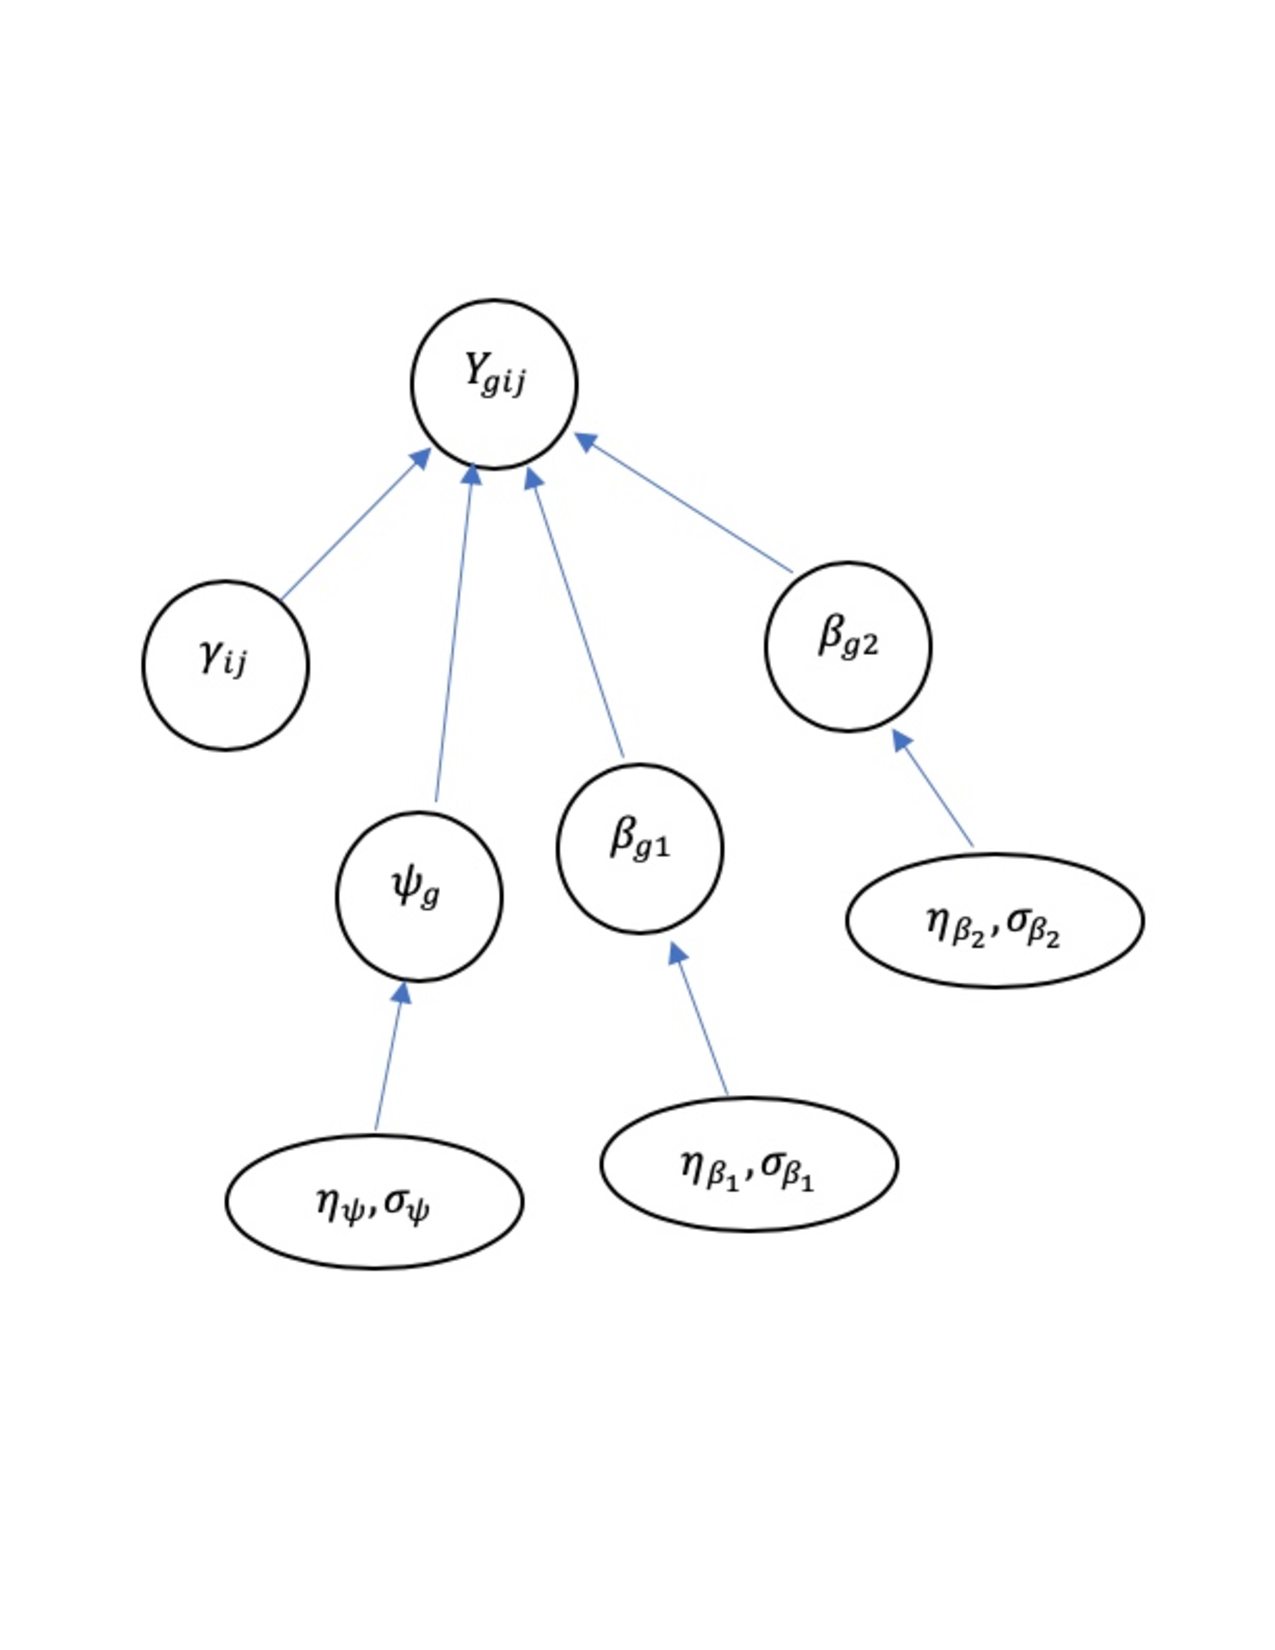
\includegraphics[scale=1, height=10cm]{dag1c}
\end{center}

\end{frame}


\begin{frame}
\frametitle{Empirical Bayes Method Posterior Probability of Parameters}

Condition on the estimated normalization factor $\hat{\gamma}$ and hyperparameters $\hat{\pi}$, we perform a Bayesian analysis to re-estimate the $\theta$ as:

\begin{equation}
\begin{split}
& p(\theta | y, \hat{\pi}, \hat{\gamma})  \propto \\ & \prod_{g=1}^{G} \prod_{i=1}^{2} \prod_{j=1}^{n_i} p(y_{gij} |\hat{\mu}_{gij}, \hat{\phi}_g ) p(\hat{\beta}_{g1} |\hat{\eta}_{\beta_1}, \hat{\sigma}^2_{\beta_1}) p(\hat{\beta}_{g2} | \hat{\eta}_{\beta_2}, \hat{\sigma}_{\beta_2}) p(\hat{\psi_g} | \hat{\eta}_{\psi}, \hat{\sigma}^2_{\psi})  
\end{split}
\end{equation}

where $\hat{\mu}_{gij}=\exp(\lambda_{gi}+ \hat{\gamma}_{ij}), \hat{\phi_g}=\exp(\hat{\psi}_g)$, and
$\hat{\beta}_{g1} \stackrel{ind}{\sim} N(\hat{\eta}_{\beta_1}, \hat{\sigma}^2_{\beta_1}), \hat{\beta}_{g2} \stackrel{ind}{\sim} N(\hat{\eta}_{\beta_2} , \hat{\sigma}^2_{\beta_2}), \psi_g \stackrel{ind}{\sim} N(\hat{\eta}_\psi, \hat{\sigma}^2_\psi)$.

\end{frame}

\begin{frame}
\frametitle{Null Hypothesis for DE Analysis}

$$H_0: \beta_{g2}=0$$ which is equivalent to $\lambda_{g1}=\lambda_{g2}$

Statistics used to do the DE analysis is based on the posterior probabilities of $\beta_{g2}$ as

$$P(DE_g|y, \hat{\pi}, \hat{\gamma}) = \min(P(\beta_{g2}<0|y, \hat{\pi}, \hat{\gamma}), P(\beta_{g2}>0|y, \hat{\pi}, \hat{\gamma}))$$
where $P(\beta_{g2}<0|y, \hat{\pi}, \hat{\gamma}) = \frac{1}{M}\sum_{m=1}^M I(\beta_{g2}^{(m)} < 0)$, and $P(\beta_{g2}>0|y, \hat{\pi}, \hat{\gamma}) = \frac{1}{M}\sum_{m=1}^M I(\beta_{g2}^{(m)} > 0)$



\end{frame}

\begin{frame}
\frametitle{Alternative Methods}

\textbf{Normalization}

{\tt edgeR} used gene-wise trimmed median of means (TMM), while {\tt DESeq, DESeq2, sSeq, EBSeq} used sample-wise size factor. \\

\textbf{Dispersion estimation}

{\tt edgeR} used Cox-Reid approximate conditional inderence (CRACI) moderate towards the mean while {\tt DESeq, DESeq2} used CRACI with focus on maximum individual dispersion estimate; {\tt sSeq} estimated dispersion by pooling all the samples using the method of moments(MM), and then shrinking the gene-wise estimates through minimizing the mean-square error; {\tt EBSeq} also estimated the gene-specific varainces via MM. \\


\textbf{Test for DE}

{\tt edgeR, sSeq} used exact test for 2 factors; {\tt DESeq, DESeq2} used Wald test for 2 factors; 

\end{frame}

\section{Simulation studies}


\begin{frame}
\frametitle{Simulation studies}

Parameter estimation use {\tt edgeR}: $\hat{\beta}_{g1}, \hat{\beta}_{g2}, \hat{\phi}_g$, and the normalized library sizes $N_{ij}$
\newline
\newline
Simulation scenario set up: nGenes, nSamples, pDiff
\newline
\newline
Simulation model: $Y_{gij} \ind \text{NB} \left (\mu_{gij}, \phi_g \right )$ with $\mu_{gij} = \exp(x_i^T\beta_g + \log(N_{ij}))$ where $N_{ij}$ is the normalized library size. For non-DE genes, we set $\mu_{g1} = \mu_{g2}$. 

\end{frame}


\section{Simulation Results}

\begin{frame}
\frametitle{ROC Curves of One Scenario}

\begin{center}
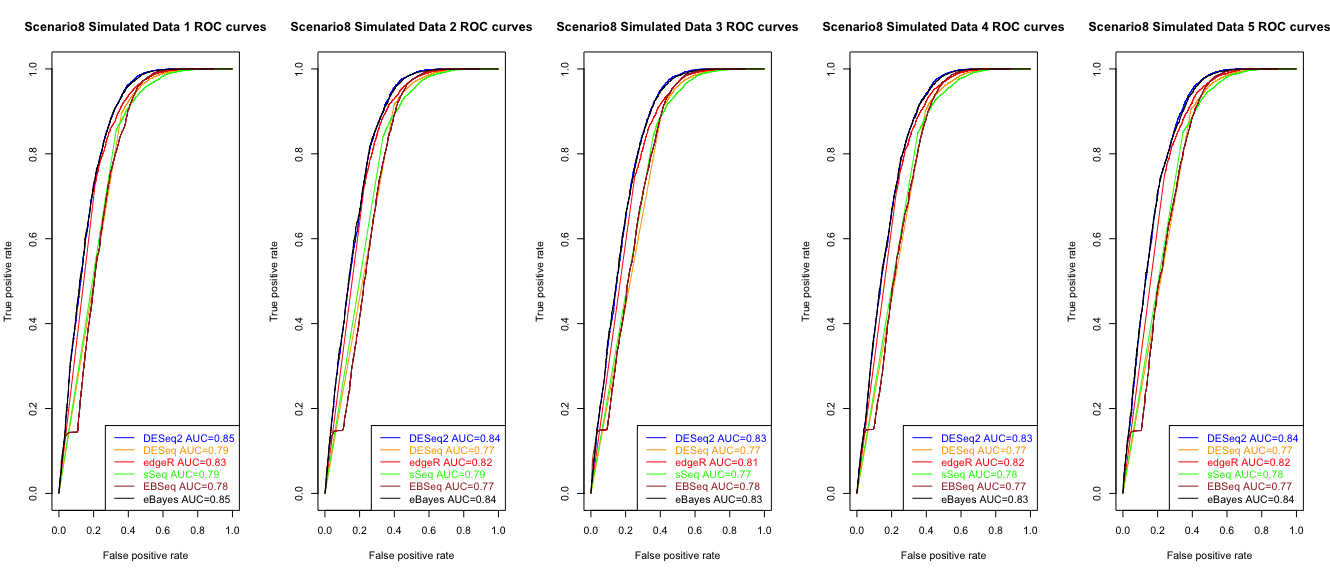
\includegraphics{sc8_roc}
\end{center}
nGenes=10000, nSample=16, pDiff=30\% Scenario ROC Curves

\end{frame}



\begin{frame}

\frametitle{AUC Plot}
\begin{center}
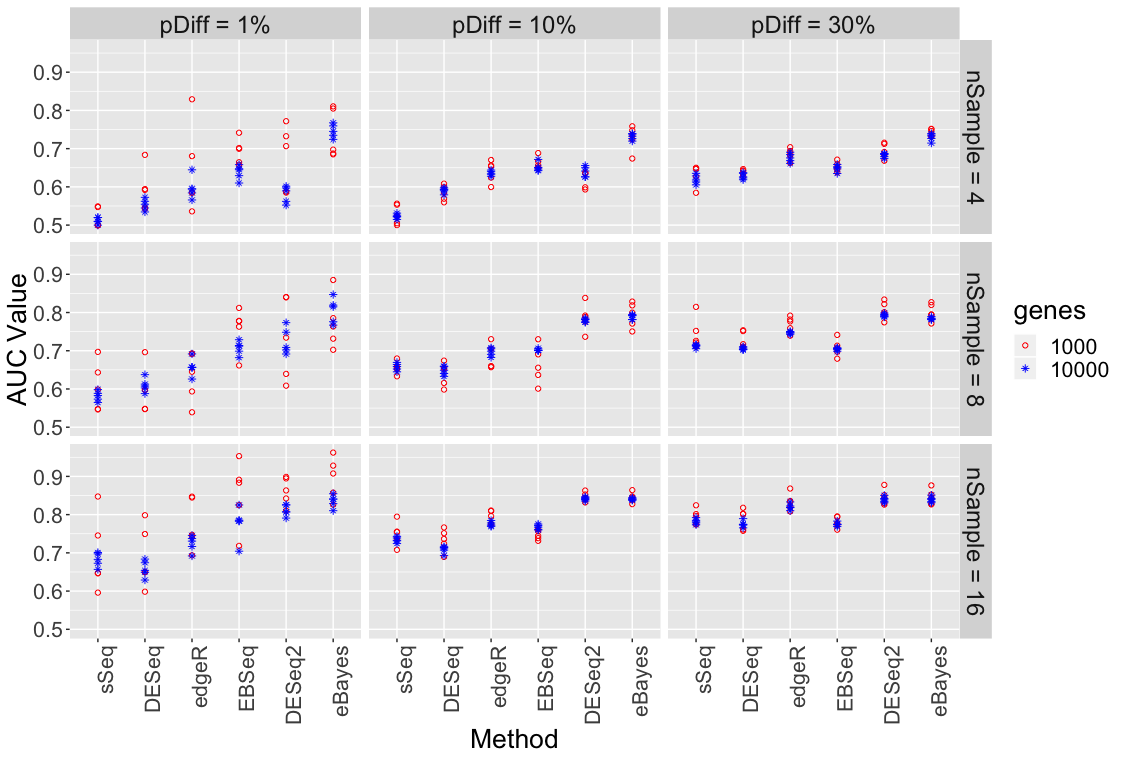
\includegraphics{auc_plot}
\end{center}

\end{frame}


\begin{frame}
\frametitle{Summary of the Results}


Effect of nGenes: not obvious
\newline
\newline
Effect of pDiff: smaller pDiff -> larger differences between {\tt eBayes} and other methods
\newline
\newline
Effect of nSample: smaller nSample -> larger differences between {\tt eBayes} and other mehods



\end{frame}

\begin{frame}
\frametitle{Discussion}

For the future research, we could:
\newline
(1) add more methods: baySeq, ShrinkSeq, NOISeq, SAMseq;\\
(2) include more varieties;\\
(3) consider the flow cell effects;\\
(4) improve the eBayes by refining the hierarchical model

\end{frame}


\end{document} 


